\documentclass[english, 11 pt, class=article, crop=false]{standalone}
\usepackage[T1]{fontenc}
%\renewcommand*\familydefault{\sfdefault} % For dyslexia-friendly text
\usepackage{lmodern} % load a font with all the characters
\usepackage{geometry}
\geometry{verbose,paperwidth=16.1 cm, paperheight=24 cm, inner=2.3cm, outer=1.8 cm, bmargin=2cm, tmargin=1.8cm}
\setlength{\parindent}{0bp}
\usepackage{import}
\usepackage[subpreambles=false]{standalone}
\usepackage{amsmath}
\usepackage{amssymb}
\usepackage{esint}
\usepackage{babel}
\usepackage{tabu}
\makeatother
\makeatletter

\usepackage{titlesec}
\usepackage{ragged2e}
\RaggedRight
\raggedbottom
\frenchspacing

% Norwegian names of figures, chapters, parts and content
\addto\captionsenglish{\renewcommand{\figurename}{Figur}}
\makeatletter
\addto\captionsenglish{\renewcommand{\chaptername}{Kapittel}}
\addto\captionsenglish{\renewcommand{\partname}{Del}}


\usepackage{graphicx}
\usepackage{float}
\usepackage{subfig}
\usepackage{placeins}
\usepackage{cancel}
\usepackage{framed}
\usepackage{wrapfig}
\usepackage[subfigure]{tocloft}
\usepackage[font=footnotesize,labelfont=sl]{caption} % Figure caption
\usepackage{bm}
\usepackage[dvipsnames, table]{xcolor}
\definecolor{shadecolor}{rgb}{0.105469, 0.613281, 1}
\colorlet{shadecolor}{Emerald!15} 
\usepackage{icomma}
\makeatother
\usepackage[many]{tcolorbox}
\usepackage{multicol}
\usepackage{stackengine}

\usepackage{esvect} %For vectors with capital letters

% For tabular
\usepackage{array}
\usepackage{multirow}
\usepackage{longtable} %breakable table

% Ligningsreferanser
\usepackage{mathtools}
\mathtoolsset{showonlyrefs}

% index
\usepackage{imakeidx}
\makeindex[title=Indeks]

%Footnote:
\usepackage[bottom, hang, flushmargin]{footmisc}
\usepackage{perpage} 
\MakePerPage{footnote}
\addtolength{\footnotesep}{2mm}
\renewcommand{\thefootnote}{\arabic{footnote}}
\renewcommand\footnoterule{\rule{\linewidth}{0.4pt}}
\renewcommand{\thempfootnote}{\arabic{mpfootnote}}

%colors
\definecolor{c1}{cmyk}{0,0.5,1,0}
\definecolor{c2}{cmyk}{1,0.25,1,0}
\definecolor{n3}{cmyk}{1,0.,1,0}
\definecolor{neg}{cmyk}{1,0.,0.,0}

% Lister med bokstavar
\usepackage[inline]{enumitem}

\newcounter{rg}
\numberwithin{rg}{chapter}
\newcommand{\reg}[2][]{\begin{tcolorbox}[boxrule=0.3 mm,arc=0mm,colback=blue!3] {\refstepcounter{rg}\phantomsection \large \textbf{\therg \;#1} \vspace{5 pt}}\newline #2  \end{tcolorbox}\vspace{-5pt}}

\newcommand\alg[1]{\begin{align} #1 \end{align}}

\newcommand\eks[2][]{\begin{tcolorbox}[boxrule=0.3 mm,arc=0mm,enhanced jigsaw,breakable,colback=green!3] {\large \textbf{Eksempel #1} \vspace{5 pt}\\} #2 \end{tcolorbox}\vspace{-5pt} }

\newcommand{\st}[1]{\begin{tcolorbox}[boxrule=0.0 mm,arc=0mm,enhanced jigsaw,breakable,colback=yellow!12]{ #1} \end{tcolorbox}}

\newcommand{\spr}[1]{\begin{tcolorbox}[boxrule=0.3 mm,arc=0mm,enhanced jigsaw,breakable,colback=yellow!7] {\large \textbf{Språkboksen} \vspace{5 pt}\\} #1 \end{tcolorbox}\vspace{-5pt} }

\newcommand{\sym}[1]{\colorbox{blue!15}{#1}}

\newcommand{\info}[2]{\begin{tcolorbox}[boxrule=0.3 mm,arc=0mm,enhanced jigsaw,breakable,colback=cyan!6] {\large \textbf{#1} \vspace{5 pt}\\} #2 \end{tcolorbox}\vspace{-5pt} }

\newcommand\algv[1]{\vspace{-11 pt}\begin{align*} #1 \end{align*}}

\newcommand{\regv}{\vspace{5pt}}
\newcommand{\mer}{\textsl{Merk}: }
\newcommand{\mers}[1]{{\footnotesize \mer #1}}
\newcommand\vsk{\vspace{11pt}}
\newcommand\vs{\vspace{-11pt}}
\newcommand\vsb{\vspace{-16pt}}
\newcommand\sv{\vsk \textbf{Svar} \vspace{4 pt}\\}
\newcommand\br{\\[5 pt]}
\newcommand{\figp}[1]{../fig/#1}
\newcommand\algvv[1]{\vs\vs\begin{align*} #1 \end{align*}}
\newcommand{\y}[1]{$ {#1} $}
\newcommand{\os}{\\[5 pt]}
\newcommand{\prbxl}[2]{
\parbox[l][][l]{#1\linewidth}{#2
	}}
\newcommand{\prbxr}[2]{\parbox[r][][l]{#1\linewidth}{
		\setlength{\abovedisplayskip}{5pt}
		\setlength{\belowdisplayskip}{5pt}	
		\setlength{\abovedisplayshortskip}{0pt}
		\setlength{\belowdisplayshortskip}{0pt} 
		\begin{shaded}
			\footnotesize	#2 \end{shaded}}}

\renewcommand{\cfttoctitlefont}{\Large\bfseries}
\setlength{\cftaftertoctitleskip}{0 pt}
\setlength{\cftbeforetoctitleskip}{0 pt}

\newcommand{\bs}{\\[3pt]}
\newcommand{\vn}{\\[6pt]}
\newcommand{\fig}[1]{\begin{figure}
		\centering
		\includegraphics[]{\figp{#1}}
\end{figure}}

\newcommand{\figc}[2]{\begin{figure}
		\centering
		\includegraphics[]{\figp{#1}}
		\caption{#2}
\end{figure}}

\newcommand{\sectionbreak}{\clearpage} % New page on each section

\newcommand{\nn}[1]{
\begin{equation}
	#1
\end{equation}
}

% Equation comments
\newcommand{\cm}[1]{\llap{\color{blue} #1}}

\newcommand\fork[2]{\begin{tcolorbox}[boxrule=0.3 mm,arc=0mm,enhanced jigsaw,breakable,colback=yellow!7] {\large \textbf{#1 (forklaring)} \vspace{5 pt}\\} #2 \end{tcolorbox}\vspace{-5pt} }
 
%colors
\newcommand{\colr}[1]{{\color{red} #1}}
\newcommand{\colb}[1]{{\color{blue} #1}}
\newcommand{\colo}[1]{{\color{orange} #1}}
\newcommand{\colc}[1]{{\color{cyan} #1}}
\definecolor{projectgreen}{cmyk}{100,0,100,0}
\newcommand{\colg}[1]{{\color{projectgreen} #1}}

% Methods
\newcommand{\metode}[2]{
	\textsl{#1} \\[-8pt]
	\rule{#2}{0.75pt}
}

%Opg
\newcommand{\abc}[1]{
	\begin{enumerate}[label=\alph*),leftmargin=18pt]
		#1
	\end{enumerate}
}
\newcommand{\abcs}[2]{
	\begin{enumerate}[label=\alph*),start=#1,leftmargin=18pt]
		#2
	\end{enumerate}
}
\newcommand{\abcn}[1]{
	\begin{enumerate}[label=\arabic*),leftmargin=18pt]
		#1
	\end{enumerate}
}
\newcommand{\abch}[1]{
	\hspace{-2pt}	\begin{enumerate*}[label=\alph*), itemjoin=\hspace{1cm}]
		#1
	\end{enumerate*}
}
\newcommand{\abchs}[2]{
	\hspace{-2pt}	\begin{enumerate*}[label=\alph*), itemjoin=\hspace{1cm}, start=#1]
		#2
	\end{enumerate*}
}

% Oppgaver
\newcommand{\opgt}{\phantomsection \addcontentsline{toc}{section}{Oppgaver} \section*{Oppgaver for kapittel \thechapter}\vs \setcounter{section}{1}}
\newcounter{opg}
\numberwithin{opg}{section}
\newcommand{\op}[1]{\vspace{15pt} \refstepcounter{opg}\large \textbf{\color{blue}\theopg} \vspace{2 pt} \label{#1} \\}
\newcommand{\ekspop}[1]{\vsk\textbf{Gruble \thechapter.#1}\vspace{2 pt} \\}
\newcommand{\nes}{\stepcounter{section}
	\setcounter{opg}{0}}
\newcommand{\opr}[1]{\vspace{3pt}\textbf{\ref{#1}}}
\newcommand{\oeks}[1]{\begin{tcolorbox}[boxrule=0.3 mm,arc=0mm,colback=white]
		\textit{Eksempel: } #1	  
\end{tcolorbox}}
\newcommand\opgeks[2][]{\begin{tcolorbox}[boxrule=0.1 mm,arc=0mm,enhanced jigsaw,breakable,colback=white] {\footnotesize \textbf{Eksempel #1} \\} \footnotesize #2 \end{tcolorbox}\vspace{-5pt} }
\newcommand{\rknut}{
Rekn ut.
}

%License
\newcommand{\lic}{\textit{Matematikken sine byggesteinar by Sindre Sogge Heggen is licensed under CC BY-NC-SA 4.0. To view a copy of this license, visit\\ 
		\net{http://creativecommons.org/licenses/by-nc-sa/4.0/}{http://creativecommons.org/licenses/by-nc-sa/4.0/}}}

%referances
\newcommand{\net}[2]{{\color{blue}\href{#1}{#2}}}
\newcommand{\hrs}[2]{\hyperref[#1]{\color{blue}\textsl{#2 \ref*{#1}}}}
\newcommand{\rref}[1]{\hrs{#1}{regel}}
\newcommand{\refkap}[1]{\hrs{#1}{kapittel}}
\newcommand{\refsec}[1]{\hrs{#1}{seksjon}}

\newcommand{\mb}{\net{https://sindrsh.github.io/FirstPrinciplesOfMath/}{MB}}


%line to seperate examples
\newcommand{\linje}{\rule{\linewidth}{1pt} }

\usepackage{datetime2}
%%\usepackage{sansmathfonts} for dyslexia-friendly math
\usepackage[]{hyperref}



\begin{document}
%\setcounter{chapter}{4}	
	
\opgt
\vspace{10pt}

\st{
\textbf{Konsumprisinder}\footnote{Hentet fra \net{https://www.ssb.no/priser-og-prisindekser/konsumpriser/statistikk/konsumprisindeksen}{ssb.no}.} \vsk

	
\parbox{0.25\linewidth}{	\begin{tabular}{c|c}
		År &  KPI \\ \hline
		2020 & 112,2\\
		2019 & 	110,8\\
		2018 &  112,2 \\
		2017&	105,5\\
		2016&	103,6\\
		2015&	100\\
		2014&	97,9\\
		2013&	95,9\\
		2012&	93,9\\
		2011&	93,3\\
		2010&	92.1\\
		2009&	89.9\\		
\end{tabular}}
\parbox{0.45\linewidth}{	\begin{tabular}{c|c}
		 &   \\ \hline
		2008&	88\\
		2007&	84.8\\
		2006&	84.2\\
		2005&	82.3\\
		2004&	81\\
		2003&	80.7\\
		2002&	78.7\\
		2001&	77.7\\
		2000&	75.5\\
		1999&	73.2\\
		1998&	71.5\\
		1997&	69.9
\end{tabular}}
}


\op{kr}
Regn ut kroneverdien i årene:\os
\textbf{a)} 1998\qquad \textbf{b)} 2014 \qquad \textbf{c)} 2017


\op{hvormye}
I 2016 var KPI 103,6. Hvor mye høyere var prisnivået i 2016 enn i 2015?

\op{elsereal}
I 2017 tjente Else 490 000 kr, mens hun i 2012 tjente 410 000 kr. I
2017 var KPI $ = $ 105,5, mens i 2012 var KPI $ = $ 93,9. I hvilket av disse årene hadde Else best råd?


\nes

\op{ser}
Fra en bank låner du 200\,000 kr med 2\% i årlig rente. Lånet skal betales tilbake som et serielån med 10 årlige terminbeløp. \os
\textbf{a)} Hva blir det årlige avdraget?\os
\textbf{b)} Hva er gjelden din etter at du har betalt sjette terminbeløp?\os
\textbf{c)} Hvor mye må du betale i renter det sjuende terminbeløp?\os
\textbf{d)} Hvor stort blir det sjuende terminbeløpet?\os 

\op{anu}
Fra en bank låner du 100\,000\,kr med 2\% årlig rente. Lånet skal betales tilbake som et annuitetslån over 15 år, og banken har da regnet ut at terminbeløpet blir 7\,783.\os

Regn ut avdrag og renter for det første terminbeløpet.

\op{serogan}
Hvilken av figurene skisserer et serielån og hvilken skisserer et annuitetslån? Forklar hvorfor.
\begin{figure}	\centering
	\subfloat[]{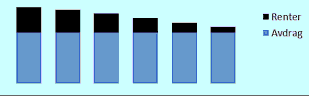
\includegraphics[scale=1]{ser}}\;
	\subfloat[]{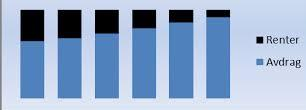
\includegraphics[scale=1]{an}}
\end{figure}

\op{spar}
Du oppretter en sparekonto i en bank som gir 2,3\% årlig rente og setter inn 45\,000\,kr. Hvor mye har du på kontoen etter 15 år?

\op{kred}
Tenk at kredittkortet ditt har 45 dagers lån uten renter, og 10\% månedlig rente etter dette. Du kjøper en scooter for 50\,000\,kr med kredittkortet. (Regn måneder som 30 dager).\os
\textbf{a)} Hvor mye skylder du banken hvis ingenting er betalt innen 75 dager?\os
\textbf{b)} Hvor mye skylder du banken hvis ingenting er betalt innen 105 dager?\os 
\textbf{c)} Hvor mye skylder du banken etter 75 dager hvis du betalte 20\,000\,kr innen de første 45 dagene?



\nes

\op{pensj}
Børge har 350\,000\,kr i lønn. Børge er pensjonist, og skal da ha 56\,000\,kr i personfradrag og 83\,000\,kr i minstefradrag. I tillegg betaler han 700\,kr i fagforeningskontigent. \os
\textbf{a)} Beregn skattegrunnlaget til Børge.\os
\textbf{b)} Av skattegrunnlaget betaler Børge 23\% skatt. Finn hvor mye dette er.

\op{miraogborge}
Mira er 19 år og tjener 200\,000 i året, mens 74 år gamle Børge tjener 350\,000 i året. \os

Hvem av de to betaler mest trygdeavgift (i antall kroner)?

\op{borge3}
Beregn trinnskatten til Børge (nevnt i oppgave \ref{pensj} og \ref{miraogborge}).

\op{borge4}
Beregn nettolønnen til Børge (nevnt i oppgave \ref{pensj}-\ref{borge3}).

\nes

\op{nora}
I februar antok Nora at dette ville bli hennes utgifter og inntekter:
\begin{itemize}
	\item 23\,000\,kr i nettolønn 
	\item 6\,000\,kr for leie av hybel
	\item 4\,500 kr på mat
	\item 1\,500\,kr på andre utgifter
\end{itemize}
\textbf{a)} Sett opp et budsjett for Noras inntekter og utgifter i februar.\os
\textbf{b)} Det viste seg at de \textsl{faktiske} utgiftene og inntektene ble disse:
\begin{itemize}
	\item 23\,000\,kr i nettolønn
	\item 6\,000\,kr for leie av hybel
	\item 5\,500 på mat
	\item Kjøp av fire FLAX-lodd som kostet 25\,kr hver.
	\item Gevinst på 1\,000\,kr fra FLAX-loddene
	\item 1\,800 på andre utgifter.
\end{itemize}
Sett opp et regnskap for Nora. Gikk hun med overskudd eller underskudd i februar? Ble overskuddet/underskuddet større eller mindre enn i budsjettet?



\end{document}